
\begin{figure}[h]
\begin{center}
\centerline{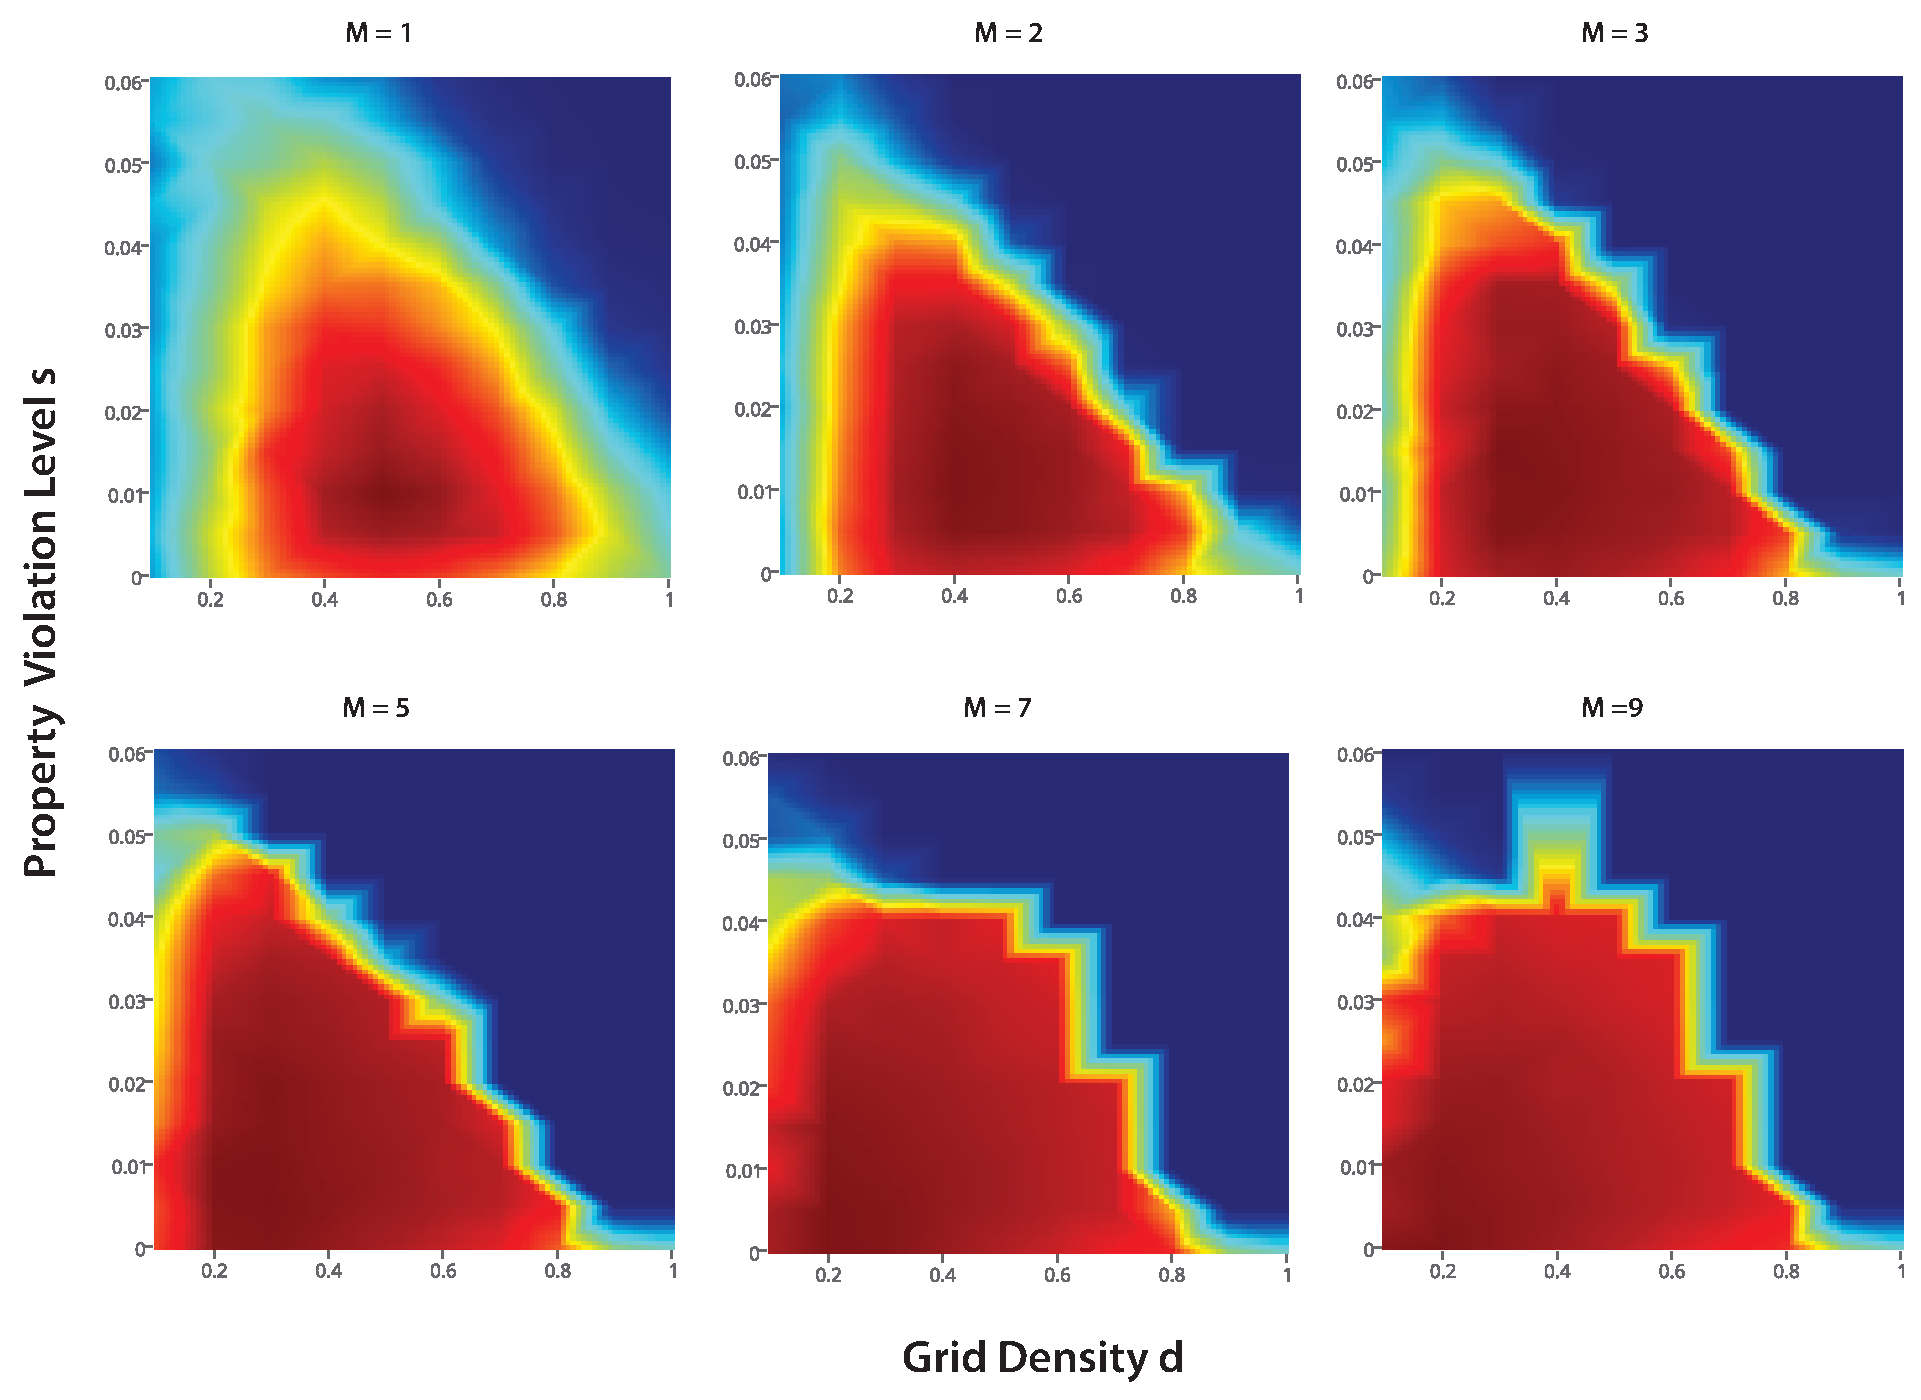
\includegraphics[width=14cm]{../figures2/heatmaps.eps}}
\caption{Cooperation levels after $N=200$ iterations [i.e., $200 \times 49^2 = 480,200$ Monte Carlo Steps (MCS)] for migration Moore's distances $M = \{1,2,3,5,7,9,11,15,20 \}$, as a function of population density $d$ and probability of property violation $s$. At initialization ($t=0$), there is a $50\%$ chance that a player will cooperate (resp. defect). The uneven landscapes reflect the statistical fluctuations of simulations. For all values of $M$, the cooperation exhibits a sharp drop for $d > d^*$  and $s > s^*$ with $(d^*,s^*)$ being a function of $M$. For high grid density ($d > 0.9$), cooperation cannot be sustained even with low property violation. As the migration range gets large $M > 9$ , the area of sustainable cooperation shrinks drastically.%(see SI Section \ref{SI:d09} for further details on {\it migration} and {\it property} games in densely populated worlds).
}
\label{fig:heatmaps}
\end{center}
\end{figure}



\begin{figure}[h]
\begin{center}
\centerline{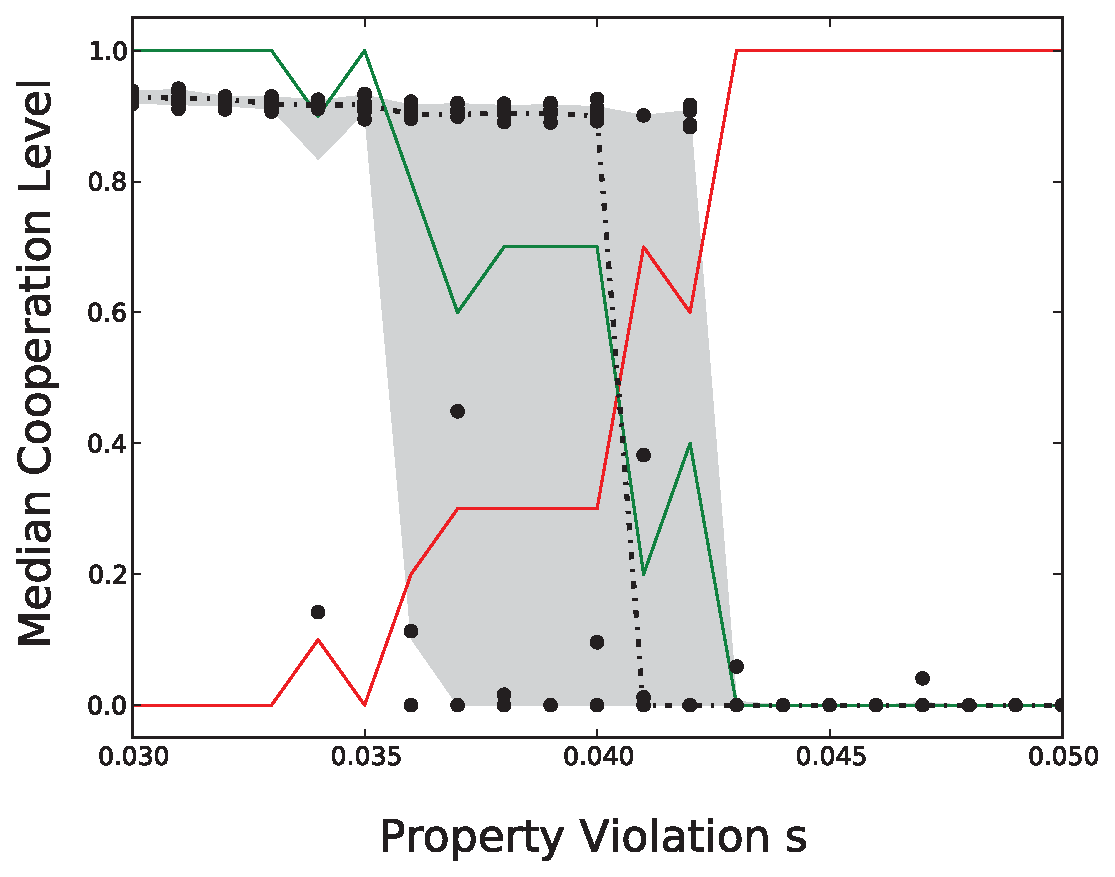
\includegraphics[width=9cm]{../figures2/phase_transition_d05_paper.eps}}
\caption{Phase transition of cooperation levels after $N=200$ iterations [i.e., $200 \times 100^2 = 2M$ Monte Carlo Steps (MCS)] for migration Moore's distance $M = 5$ and population density $d=0.5$. The cooperation level (dotted black line) exhibits a sharp drop around $0.035 < s^{*} < 0.044$, with an equal probability that cooperative players will strive or disappear around $s^{*} \approx 4.01\times10^{-2}$: Probabilities that cooperative players invade the grid ($> 0.8$) or disappears ($< 0.2$) are shown (green and red lines). The cooperation is stochastic and does not depend on the initial grid configuration}
\label{fig:comparison_no_with_migration}
\end{center}
\end{figure}




%\begin{figure}[h]
%\begin{center}
%\centerline{\includegraphics[width=9cm]{../figures/configurations_t200.eps}}
%\caption{Grid configurations at $t=200$, with fully rational agents (probability of imitation $m=1$), and grid density $d=0.5$. When there is no migration $M=0$ (and {\it a fortiori} no property violation $s=0$) (see {\it A.}), clusters of cooperators can only form by local influence, and the simulation is quickly frozen. As the migration range increases, larger clusters form when cooperators (see {\it B.,E.}) or defectors (see {\it D.,G.}) win. At the lower limit of the phase transition point $s \rightarrow s^{*}_{-}$, cooperators form clusters, which stay strong (large?) enough to keep defectors at bay (see {\it C.,F.}). When $s > s^{*}_{+}$ cooperation cannot survive. However, with larger migration range $M=5$, the transition point $s^*$ is almost three times larger, compared to $M=1$.}
%\label{fig:configurations_t200}
%\end{center}
%\end{figure}
%
%
%\begin{figure}[h]
%\begin{center}
%\centerline{\includegraphics[width=11cm]{../figures/configurations_t200_M11plus.eps}}
%\caption{Grid configurations at $t=200$, with fully rational agents (probability of imitation $m=1$), and grid density $d=0.5$ in the case of large migration ranges ($M = \{11,13\}$). For $M$ large enough, two distinct transition points appear ($s^{*}_{-}$ and $s^{*}_{+}$), with an intermediary stable state (see {\it C.} and {\it G.}), where cooperators are in minority ($c = 0.45\pm0.05$), yet their clusters resistant to defector invasions. Note that configurations look the same for $M=11$ and $M=13$, but the transition interval $(s^{*}_{-}$,$s^{*}_{+}$ has slightly larger values in the latter case, suggesting that populations with larger migration range can sustain more property violation.}
%\label{fig:configurations_t200_M11plus}
%\end{center}
%\end{figure}


%\begin{figure}[h]
%\begin{center}
%\centerline{\includegraphics[width=11cm]{../figures/configurations_t200.eps}}
%\caption{Grid configurations at $t=200$, with fully rational agents (probability of imitation $m=1$), and grid density $d=0.5$. When no migration (and {\it a fortiori} no property violation) is present (see {\it A.}), clusters of cooperators can only form by local influence, and the simulation is quickly frozen. As the migration range increases,  larger clusters form when cooperators (see {\it B.,E.}) or defectors (see {\it D.,G.}) win. At the lower limit of the phase transition point $s \rightarrow s^{*}_{-}$, cooperators form clusters, which stay strong (large?) enough to keep defectors at bay (see {\it C.,F.}).}\label{fig:comparison_no_with_migration}
%\end{center}
%\end{figure}




%\begin{figure}[h]
%\begin{center}
%\centerline{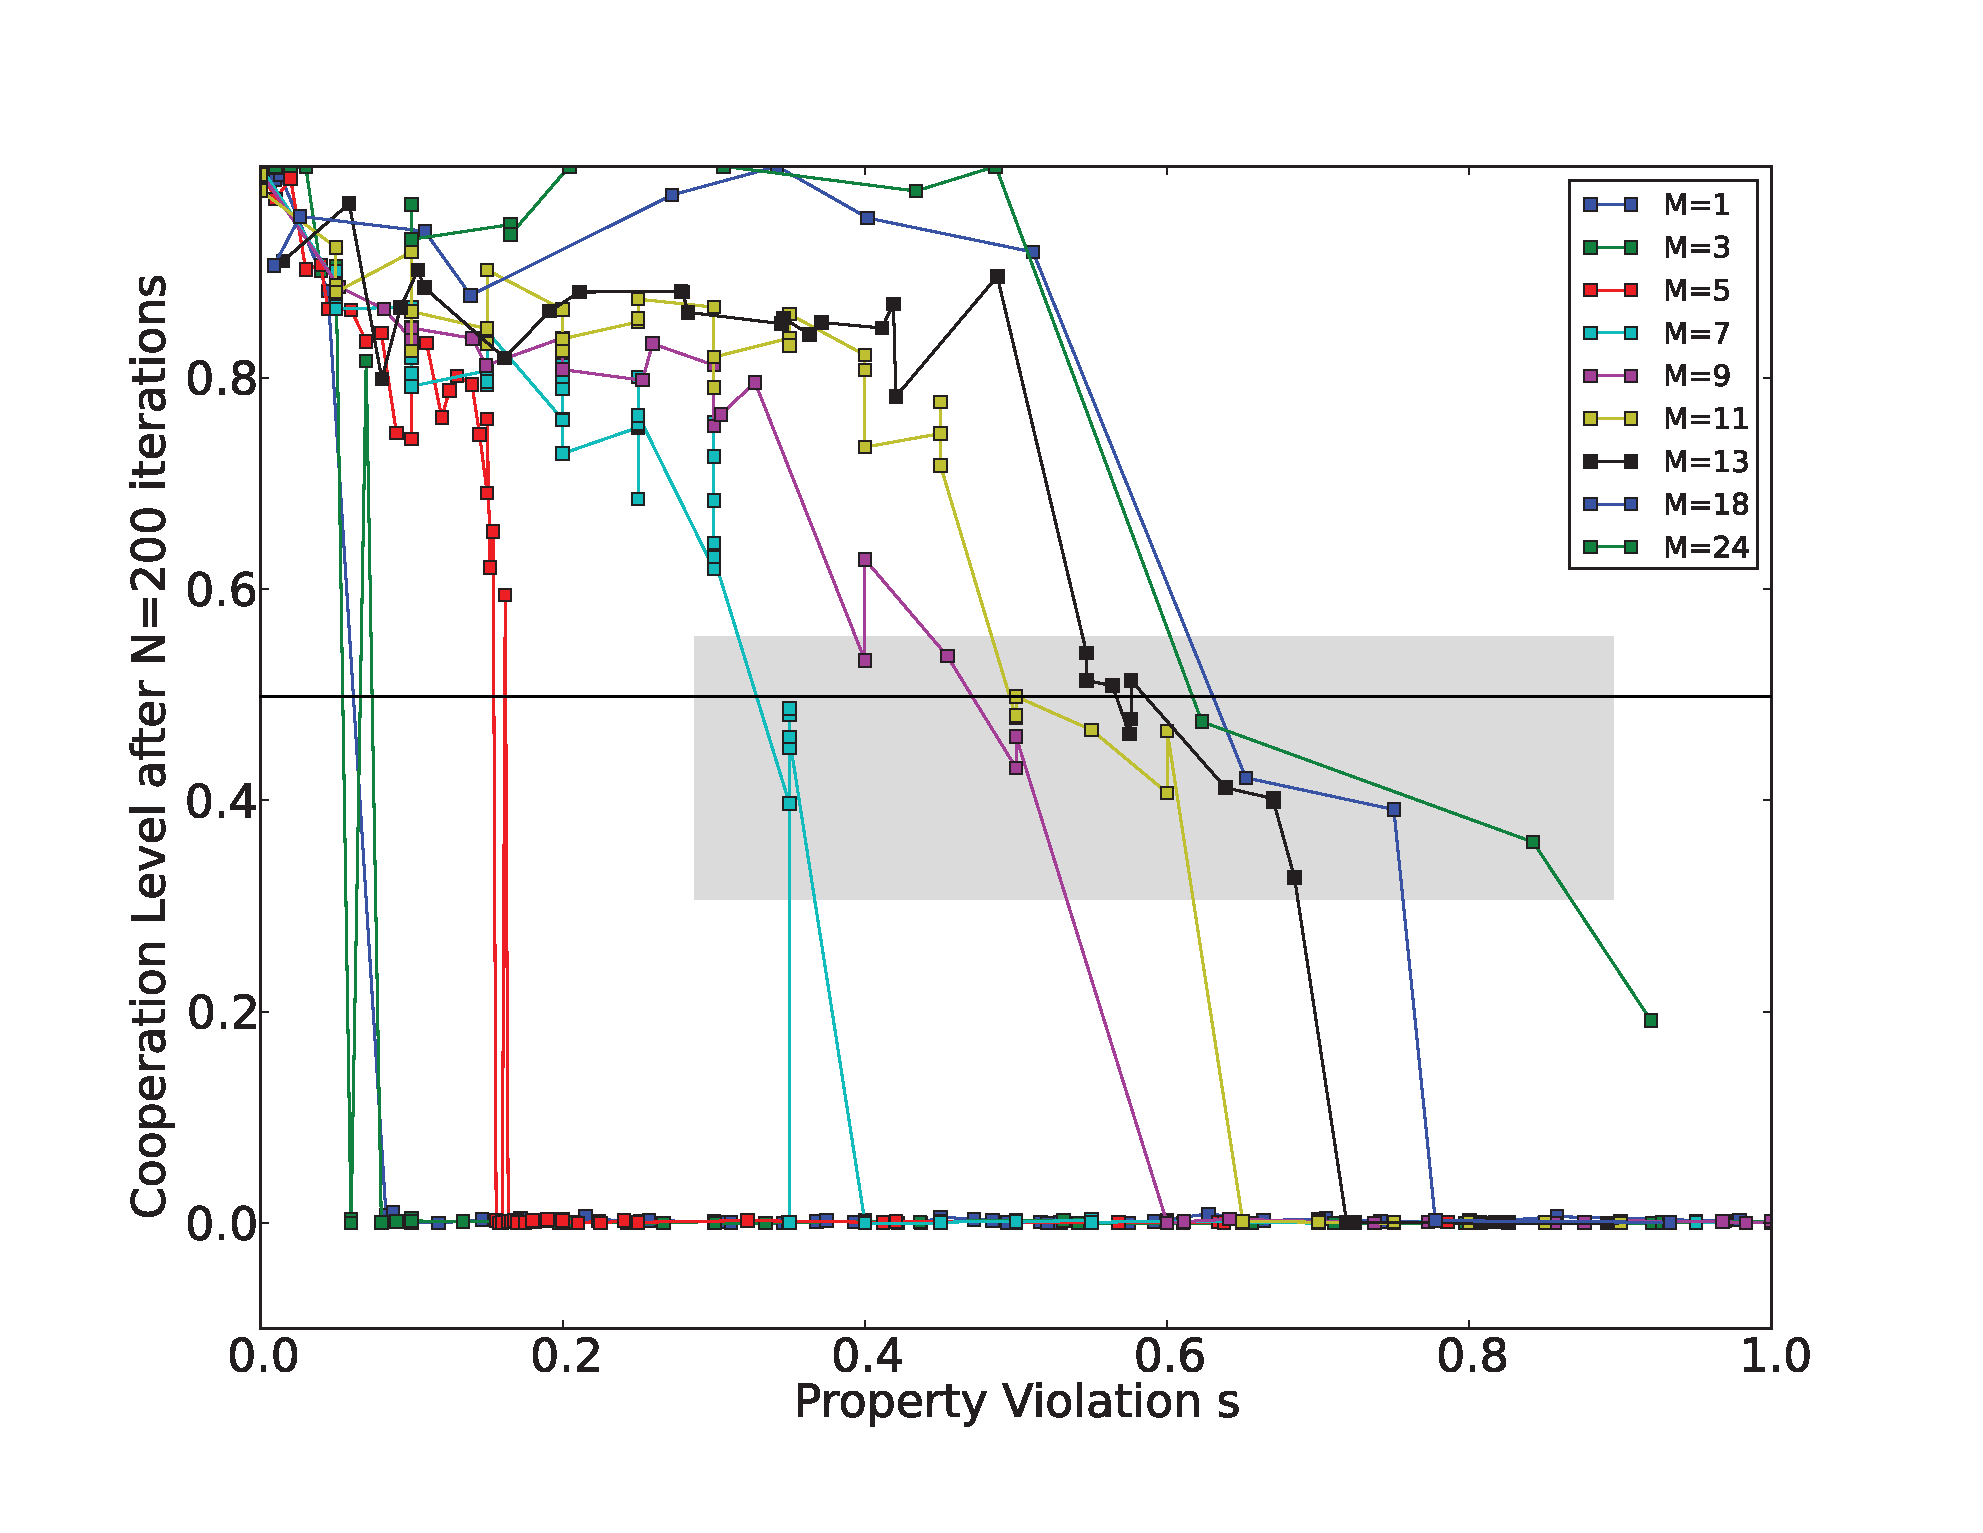
\includegraphics[width=15cm]{../figures/phase_transitions_2.eps}}
%\caption{Typical phase transitions for migration ranges $1 \leqslant M \leqslant 24$ ($0.4 \leqslant d < 0.6$). When there is no property violation $s = 0$, cooperators invade the world for any migration range $M > 0$. For small $M = \{ 1,3,5\}$, a sharp phase transition occurs at a transition point $s^{*}$, from a high level of cooperators in the populations ($c > 0.6$) when $s < s^{*}$ to entire collapse of cooperators for $s > s^{*}$. For $M \leqslant 5$, there is no intermediary state, whereas for $M \geqslant 7$, an intermediary state appears defined by $s^{*}_{-} < s < s^{*}_{+}$, with populations of cooperators in minority ($c \approx 0.45 < 0.5$) compared to defectors. For $M= \{ 7,9\}$, there is a non-zero probability of cooperation collapse, while for larger migration ranges ($M \geqslant 11$), this intermediary state becomes more stable, i.e., process converges almost surely  {\bf [to be further checked]}. Larger migration ranges increase both the maximum number of cooperators when $0 < s < s^{*}_{-}$, increase the lower $s^{*}_{-}$ and higher $s^{*}_{+}$ bounds of property violations, below (resp. above) which cooperative populations win (resp. disappear), and decreases the minimum average proportion of cooperative populations needed in order for cooperation to strive {\bf [to be further checked]}.}
%\label{fig:phase_transition}
%\end{center}
%\end{figure}








%
%
%\begin{figure}[h]
%\begin{center}
%%\centerline{\includegraphics[width=12cm]{Figures/CCDF_A.eps}}
%\caption{Representative spatial organizations for the {\it property game}: {\bf a.} Cooperation can be maintained despite 20\% of property violation probability $(M,d,s) = (9,0.5,0.2)$, {\bf b.} Cooperation collapses quickly for $s>s^*$  $(M,d,s) = (5,0.5,0.5)$, {\bf c.} and {\bf d.} phase transition at $s^{*} = 0.155\pm0.5$ and cooperation can be maintained or on the contrary collapse {\bf [discuss how it may be only a question of time before collapse $\rightarrow$ further simulations + stochastic considerations?]}, {\bf e.} Considerations for $(M,d,s) = (1, 0^+,0.5)$ (c.f. upper left panel Figure \ref{fig:cooperation_M}), and {\bf f.} Considerations for $(M,d,s) = (7,0.9,0^+)$.}
%\label{fig:configurations}
%\end{center}
%\end{figure}

